% Front matter of the Thesis
% Title page
% Loughborough University Thesis Access Form
% Loughborough University Certificate of Originality
% Abstract
% Acknowledgements
\title{\bf Building BT Network}

\author{by\\
Zhihao DAI\\
Yunsong ZHANG\\
Huijing LEI\\
Changrong CHEN\\
Yan HUANG\\
\\
{\bf 19COP502 Building Secure Networks}\\
{\bf Lab Report}\\
\\
Loughborough University\\
\\
\copyright
\hspace{1 dd} BT NETWORK 2019\\
\\
Nov. 2019
}
\date{} % Used to remove date from title so it can be set at any date rather than the current date

\maketitle

% Set page numbers to roman numerals for front matter
\pagenumbering{roman}

% % PDF exports of Word Documents available (Exported August 2012)
% % Thesis Access Form
% 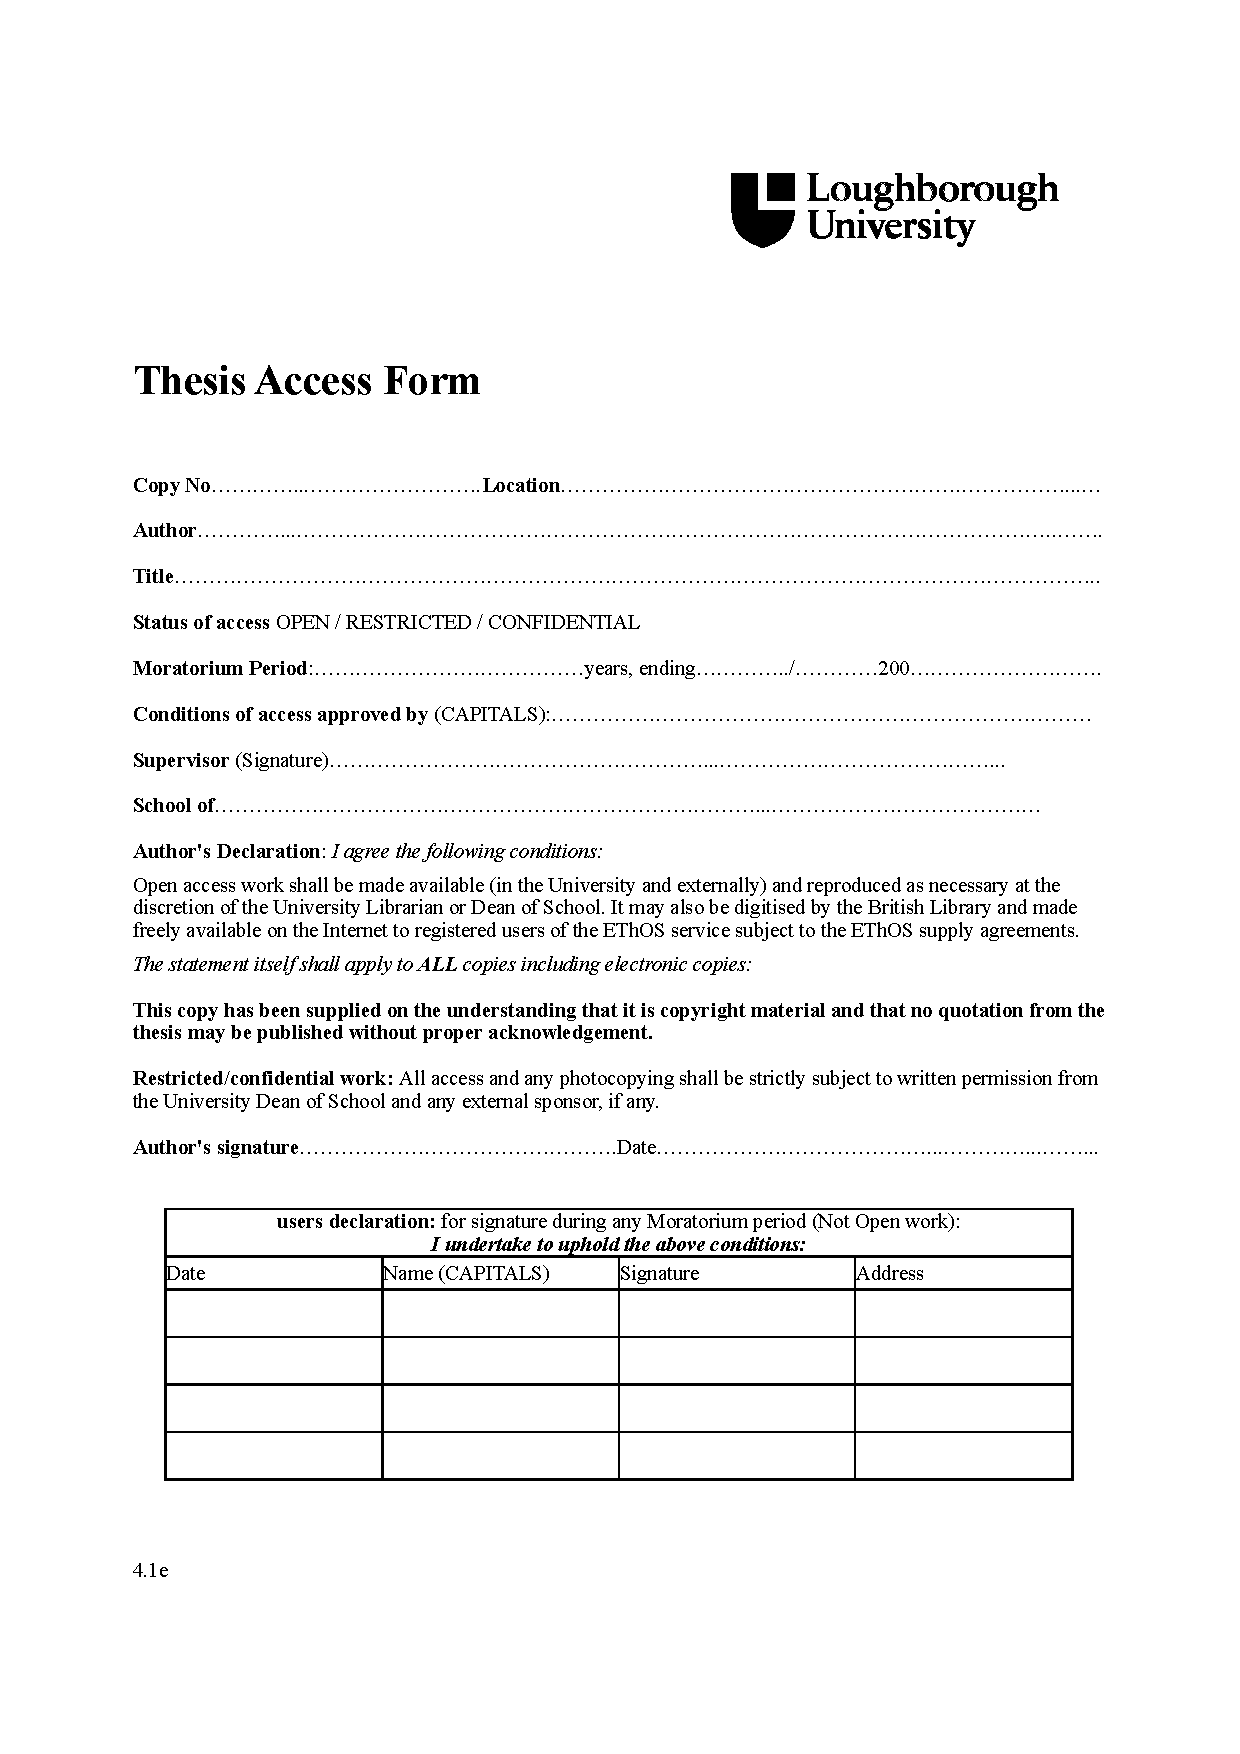
\includepdf[pages=1, pagecommand=, templatesize={5in}{10in}]{Front/LU/access.pdf}
% % Certificate of Originality
% 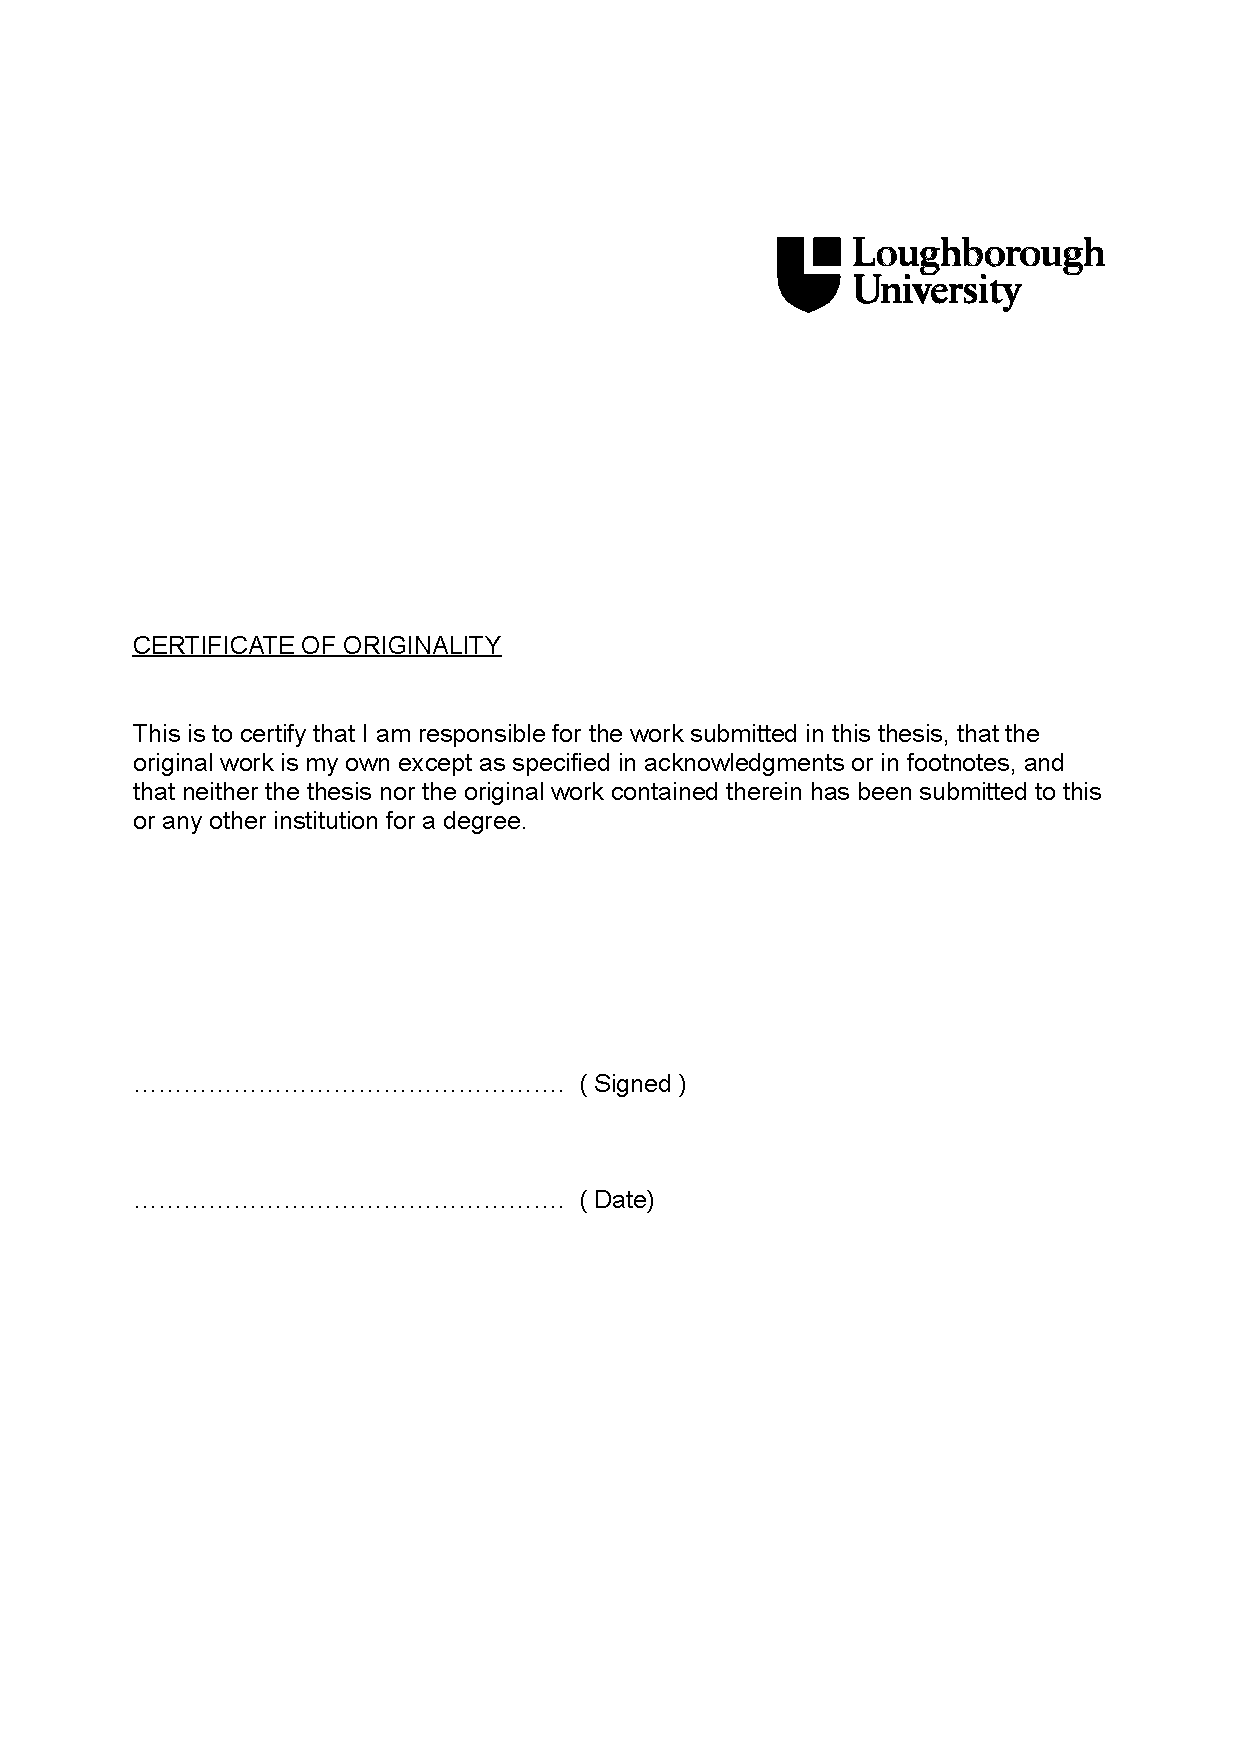
\includepdf[pages=-, pagecommand=, templatesize={5in}{10in}]{Front/LU/origin.pdf}

% Abstract
\addcontentsline{toc}{chapter}{Abstract}
\chapter*{Abstract}
This report describes the building process of BT Network, a small version of Tier-2 Internet Service Provider.
To first define the architecture of the network, a network diagram is drawn, in which physical connections are established and IP addresses are assigned. 
Then, connectivity within the network and with outside networks are made possible through internal routing protocol Intermediate System to Intermediate System (IS-IS) and external Border Gateway Protocol (BGP).
In addition, services such as World Wide Web (WWW), Domain Name System (DNS) and Email are provided in the network.
At last, main conclusions and further improvements are discussed.

% % Acknowledgements
% \addcontentsline{toc}{chapter}{Acknowledgements}
% \chapter*{Acknowledgements}
% Acknowledgement section.

% Set the depth for your table of content
% Currently set at 2 (Chapter, Section, Subsection)
\setcounter{tocdepth}{2}
% Include a table of content
\tableofcontents

% Include a list of figures
\addcontentsline{toc}{chapter}{List of Figures}
\listoffigures

% Include a list of tables
\addcontentsline{toc}{chapter}{List of Tables}
\listoftables

% Include a list of Listings
\addcontentsline{toc}{chapter}{List of Listings}
\renewcommand*{\lstlistlistingname}{List of Listings}
\lstlistoflistings

% Include a list of abbreviations using nomenclature package
%\addcontentsline{toc}{chapter}{List of Abbreviations}
%\printnomenclature[3cm] 

\newpage

% Set page numbering to arabic for body of Thesis
\pagenumbering{arabic}
